% ---
% Reemplaza líneas 3458–3462 de Docs/Technical_Report.tex.
% Decisiones y hallazgos que lo respaldan: D-038, H-044, H-045, H-046, H-047, H-048.
% ---

\subsection{Clasificadores de kernel y búsqueda de ventaja}

% fuente: H-044; X4_test.csv, X4_test_diferencias.csv
Para dilucidar si el rendimiento inferior observado en el perceptrón multicapa obedece a la codificación cuántica de los datos o al método de lectura, se evaluó un clasificador de vectores de soporte con kernel cuántico (QSVM) con regularización $C = 1$ y escala fija $c = 1$. En el conjunto de prueba oficial, el SVM clásico con kernel de base radial (RBF) alcanza un AUC-ROC de 0.649 [IC 95\,\%: 0.57, 0.73] en masas y de 0.769 [0.70, 0.83] en calcificaciones. El QSVM evaluado sobre el kernel cuántico de la condición C4 obtiene 0.628 [0.55, 0.70] en masas y 0.759 [0.69, 0.83] en calcificaciones, mientras que con el kernel de C5 logra 0.599 [0.52, 0.68] y 0.701 [0.62, 0.78]. La diferencia pareada entre el QSVM sobre C4 y el SVM RBF clásico resulta estadísticamente indistinguible de cero: $-0.02$ [$-0.05$, $0.01$] en masas y $-0.01$ [$-0.04$, $0.02$] en calcificaciones.

% fuente: H-044; X4_test.csv, X4_test_diferencias.csv
En contraste, al comparar el QSVM sobre el kernel de C4 frente al clasificador entrenado sobre las expectativas locales $\langle Z_i \rangle$ de C4 (AUC de 0.530 [0.47, 0.59] en masas y 0.633 [0.56, 0.70] en calcificaciones), el QSVM supera al modelo sobre expectativas en $+0.10$ [$0.03$, $0.17$] en masas y en $+0.13$ [$0.05$, $0.20$] en calcificaciones. Esta evidencia demuestra que la codificación cuántica en el espacio de Hilbert preserva prácticamente la totalidad de la información diagnóstica; la degradación ocurre en la etapa de lectura al proyectar un estado de 4\,096 amplitudes complejas en solo 12 valores esperados locales tras un circuito variacional fijo. Al optimizar la escala angular $c$ por validación cruzada, el QSVM con C4 iguala al mejor kernel clásico en el conjunto de prueba (diferencias de $-0.002$ en masas con $c = 0.05$ y $-0.005$ en calcificaciones con $c = 0.2$), en concordancia con el valor moderado de la diferencia geométrica ($g \approx 1.4 \ll \sqrt{N}$) formulada por Huang et al. \cite{huang2021power}.

\begin{figure}[htbp]
\centering
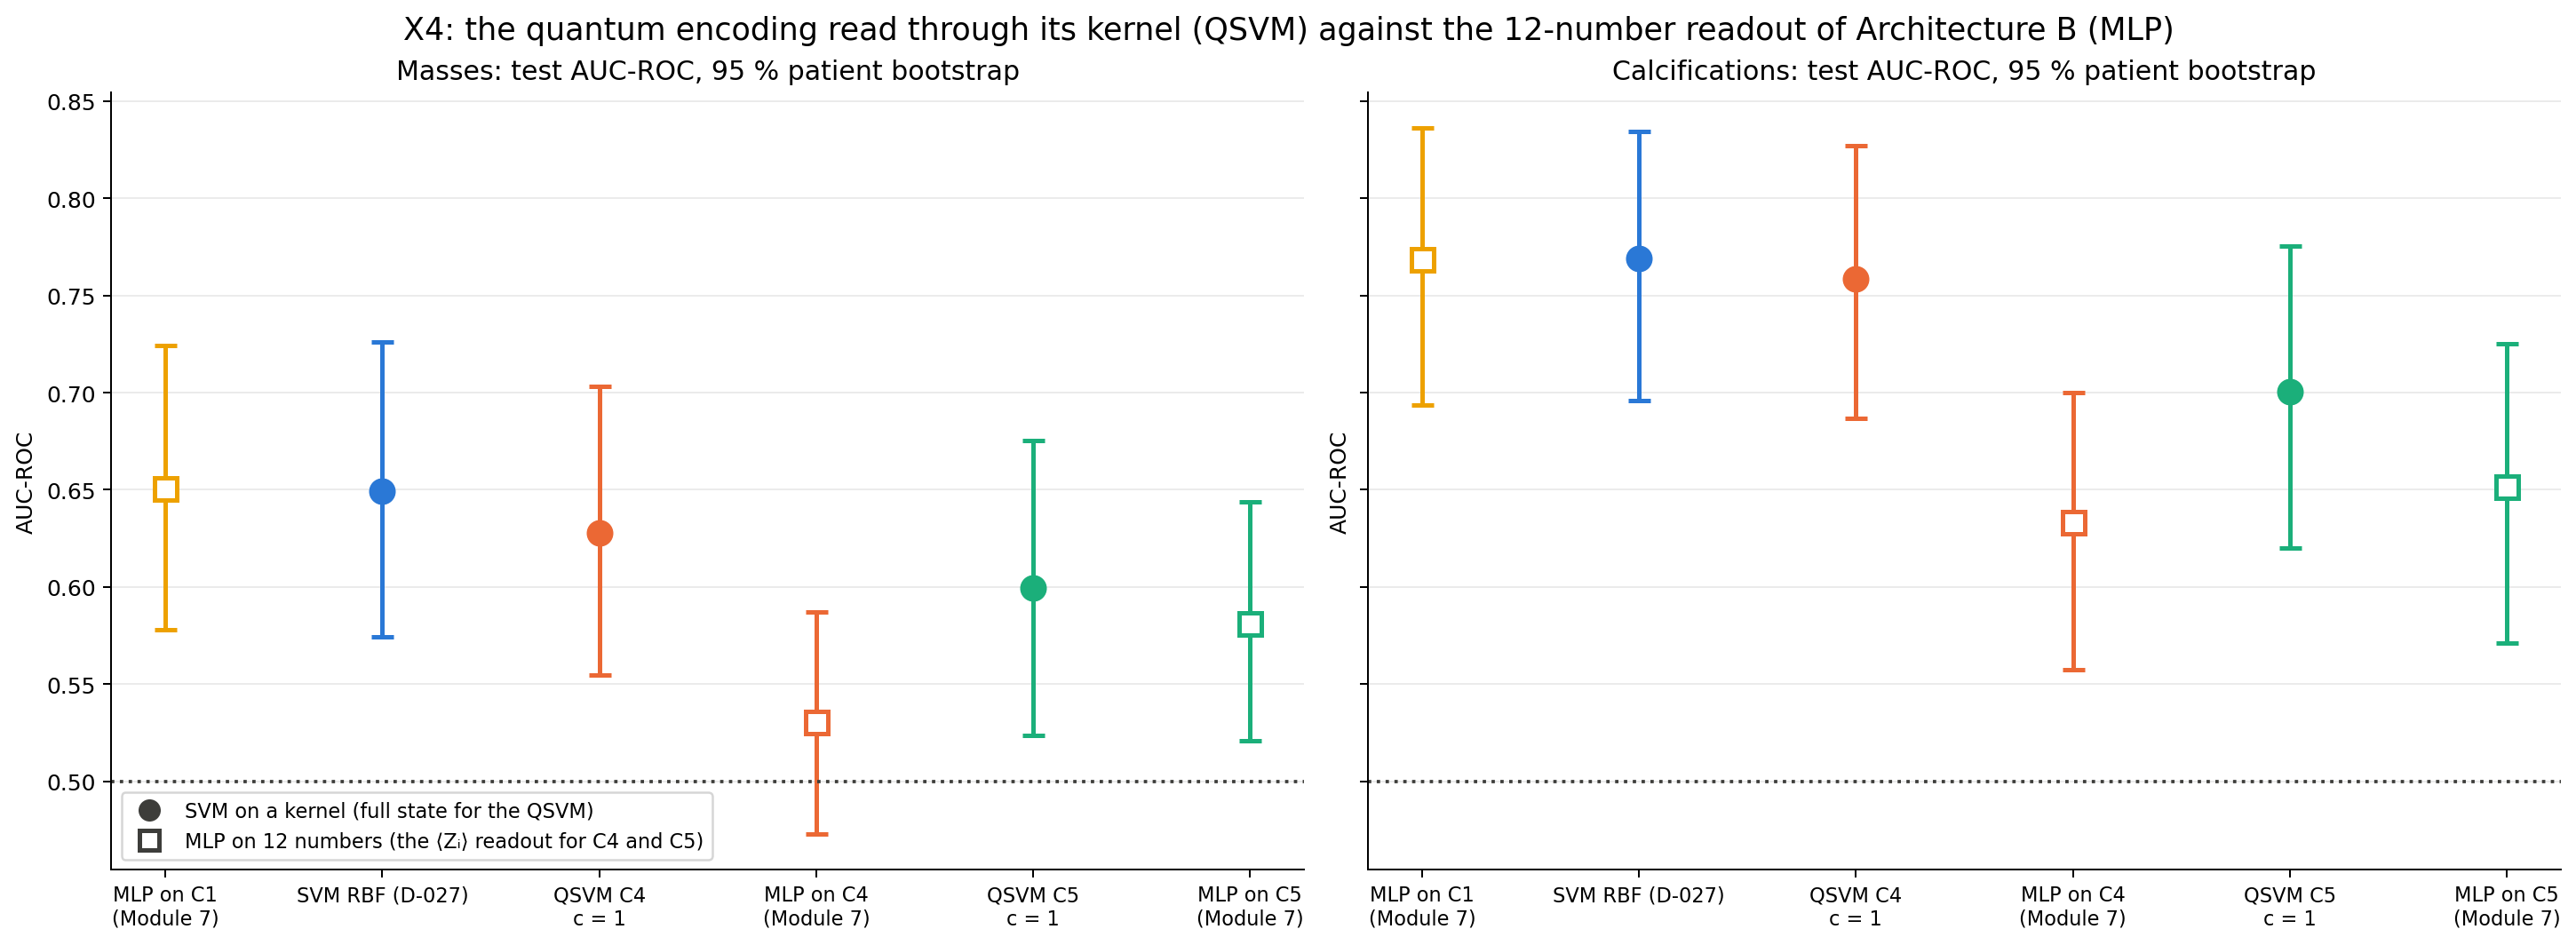
\includegraphics[width=\textwidth]{Figures/X4_qsvm_vs_readout.png}
\caption{Comparación entre el clasificador de kernel cuántico (QSVM), el clasificador de vectores de soporte clásico (SVM RBF) y la lectura mediante expectativas locales $\langle Z_i \rangle$ con red neuronal.}
\label{fig:x4_qsvm_vs_readout}
\end{figure}

% fuente: H-045; X4_67_features.csv, X4_test.csv, X4_test_diferencias.csv
La evaluación exploratoria incorporando la totalidad de las 67 características radiómicas extraídas tampoco evidencia ventaja computacional cuántica. El clasificador SVM RBF clásico sobre las 67 características obtiene un AUC de 0.649 en masas (diferencia de $-0.001$ frente a las 12 variables seleccionadas) y de 0.787 [0.73, 0.85] en calcificaciones ($+0.02$ [$-0.02$, $0.06$]). La codificación en amplitudes cuánticas sobre 7 qubits genera una matriz de kernel idéntica al cuadrado de la similitud coseno (un kernel polinomial clásico de segundo grado, con discrepancia numérica de $2 \times 10^{-16}$); este mapa alcanza un AUC de 0.795 [0.73, 0.85] en calcificaciones (sin superar significativamente al RBF clásico, con diferencia de $+0.008$) y de 0.599 en masas (diferencia de $-0.05$ [$-0.10$, $0.00$]). Por su parte, la codificación angular en producto tensorial sobre 67 qubits se concentra enteramente a escala $c = 1$ (mediana fuera de la diagonal de 0.0000), mientras que a escalas reducidas $c$ aproxima analíticamente a un kernel gaussiano clásico ($\prod \cos^2(c \Delta_i) \approx \exp(-c^2 \|\Delta\|^2)$) rindiendo a la par del SVM clásico. Un mapa con entrelazamiento completo sobre 67 variables requeriría simular $2^{67} \approx 1.5 \times 10^{20}$ amplitudes, resultando intratable clásicamente e inaccesible físicamente debido a la concentración exponencial \cite{Thanasilp2024}.

\begin{figure}[htbp]
\centering
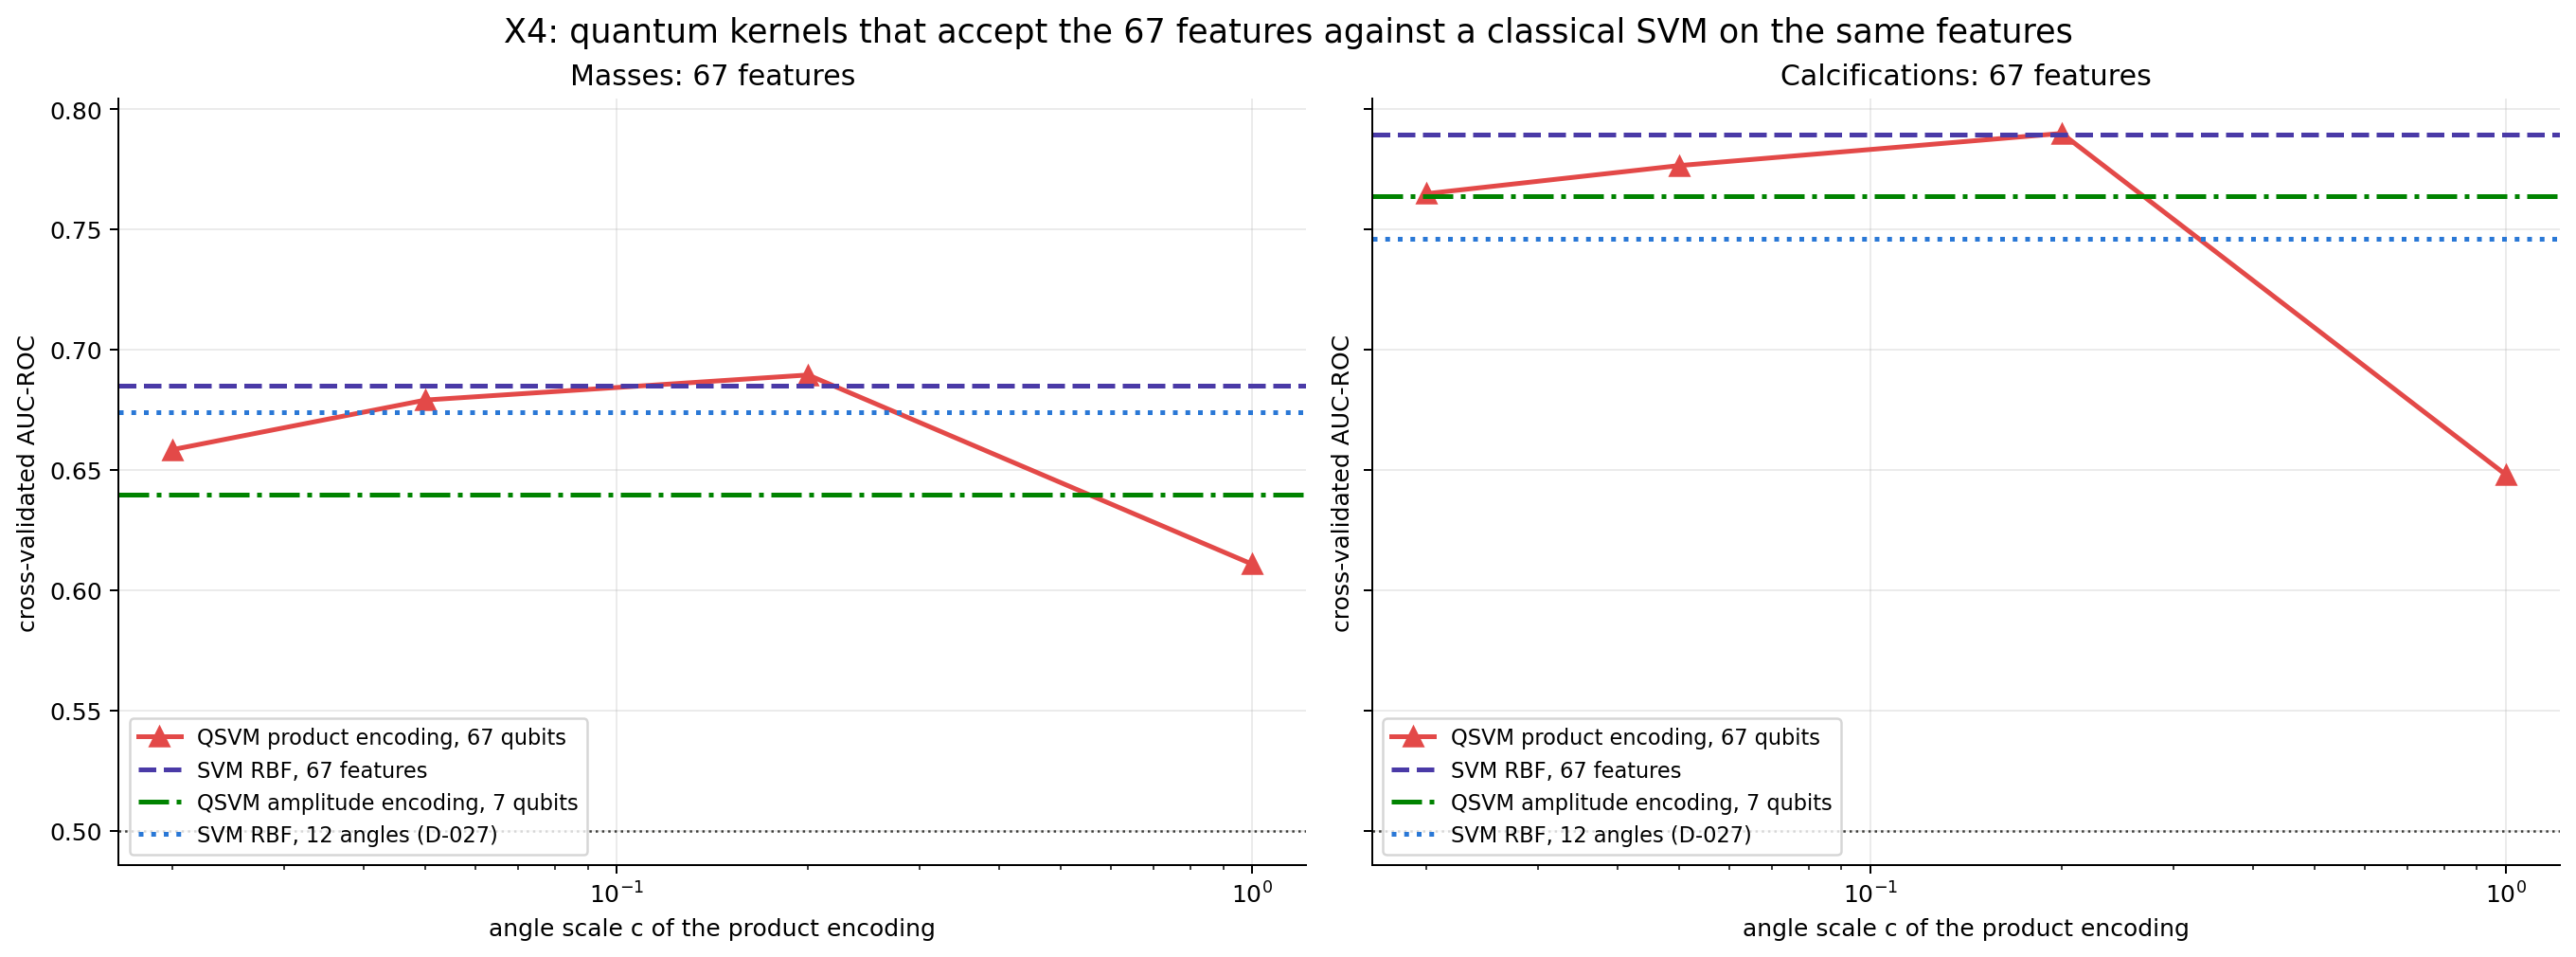
\includegraphics[width=\textwidth]{Figures/X4_67_features.png}
\caption{Rendimiento de clasificación en el conjunto de prueba al emplear las 67 características radiómicas bajo kernels clásicos, codificación en amplitudes y mapas angulares.}
\label{fig:x4_67_features}
\end{figure}

% fuente: H-046; X5_auditoria.csv
Con el fin de verificar que la ausencia de ventaja cuántica no se deba a anomalías de implementación, se llevó a cabo una auditoría del pipeline experimental, que superó las 25 verificaciones programadas. Estas pruebas confirmaron la integridad de las particiones y etiquetas de los 3\,568 casos reconstruidos directamente desde los metadatos originales sin filtración entre conjuntos, la reproducibilidad analítica del kernel cuántico por circuitos frente al cálculo por vectores de estado ($6 \times 10^{-11}$), la concordancia idéntica entre la implementación propia de SVM y la librería Qiskit Machine Learning, y la invarianza del kernel ante permutaciones de variables. Aunque dicha auditoría interna fue formulada por el propio equipo de trabajo, la reproducibilidad externa queda respaldada por la re-ejecución automatizada e integral del pipeline en un entorno limpio independiente, en la cual cero cuadernos presentaron fallos y los 81 archivos de resultados junto con los 10\,704 archivos de imágenes preprocesadas resultaron idénticos bit a bit.

% fuente: H-047; X6_anidada.csv, X6_diferencias.csv, X6_test.csv, X6_rejilla_candidatos.csv
Bajo un protocolo simétrico de validación cruzada anidada (tres pliegues internos por paciente) diseñado para buscar activamente ventaja cuántica, se contrastaron familias extendidas de kernels cuánticos y clásicos. En este procedimiento se evaluó un conjunto asimétrico compuesto por 28 candidatos cuánticos frente a 12 clásicos (140 frente a 60 ajustes considerando los pliegues de validación), una asimetría deliberada que favorece la exploración del espacio de hipótesis cuántico frente al clásico y otorga un carácter conservador a los hallazgos. En validación cruzada anidada, los contendientes clásico y cuántico alcanzan un AUC de 0.677 frente a 0.651 en masas (diferencia de $-0.027$ [$-0.043$, $-0.009$]) y de 0.745 frente a 0.753 en calcificaciones ($+0.007$ [$-0.007$, $0.023$]). En la evaluación final sobre el conjunto de prueba, el mejor modelo clásico y el mejor modelo cuántico arrojan 0.652 frente a 0.656 en masas ($+0.004$ [$-0.023$, $0.033$]) y 0.760 frente a 0.755 en calcificaciones ($-0.005$ [$-0.032$, $0.022$]).

% fuente: H-047; X6_anidada.csv, X6_diferencias.csv, X6_geometria.csv
La configuración cuántica óptima seleccionada por el procedimiento anidado converge a la equivalencia funcional con el kernel clásico: selecciona el mapa ZZ completo con escala reducida ($c = 0.05$ y $c = 0.2$), régimen en el que los términos de entrelazamiento de segundo orden se vuelven despreciables y el comportamiento emula un kernel RBF clásico. Por su parte, la hipótesis de que un entrelazamiento lineal reduciría la concentración de fidelidades resultó refutada: la mediana del kernel se reduce a 0.0001 (frente a 0.002 en el mapa completo), aproximando estados producto cuya fidelidad decae exponencialmente. Asimismo, los kernels proyectados propuestos por Huang et al. \cite{huang2021power}, si bien elevan la diferencia geométrica $g$ a un rango de 6 a 9 y la dimensión efectiva a aproximadamente 10, obtienen el desempeño clasificatorio más deficiente sobre las etiquetas clínicas reales (AUC inferior en $-0.11$ en masas y $-0.06$ en calcificaciones respecto a los clásicos), confirmando que una separación geométrica elevada es condición necesaria pero no suficiente para obtener ventaja en generalización.

\begin{figure}[htbp]
\centering
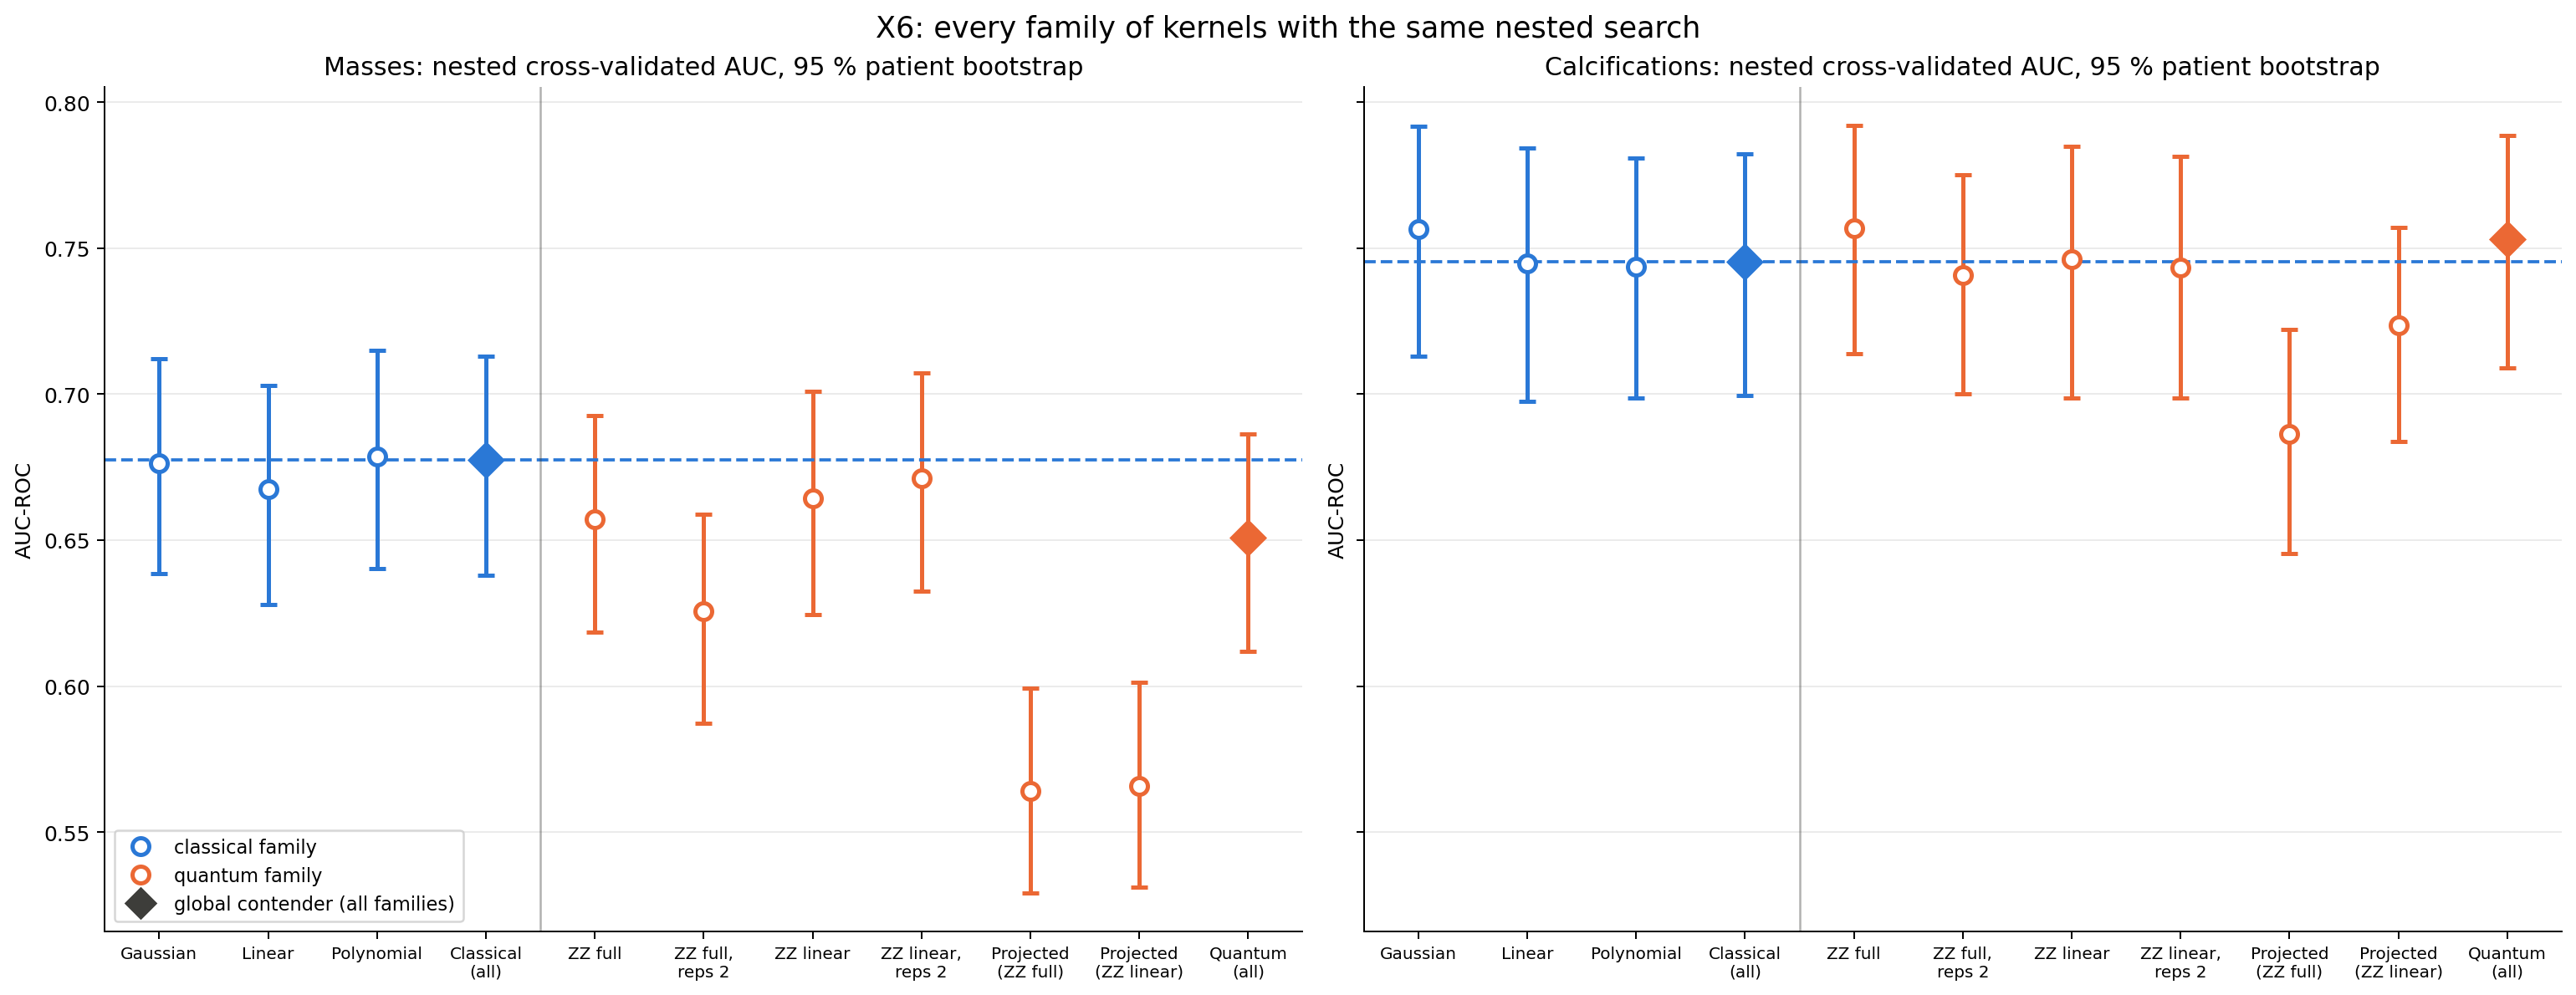
\includegraphics[width=\textwidth]{Figures/X6_nested_auc.png}
\caption{Búsqueda anidada sistemática de ventaja computacional cuántica: curvas de rendimiento en validación cruzada interna y evaluación pareada en el conjunto de prueba oficial.}
\label{fig:x6_nested_auc}
\end{figure}

% fuente: H-048; X6_etiquetas_construidas.csv
Para esclarecer si la ausencia de ventaja obedece al protocolo clasificatorio o a la estructura intrínseca del problema, se sintetizaron etiquetas artificiales alineadas geométricamente con el kernel cuántico conforme al procedimiento del Apéndice G de Huang et al. \cite{huang2021power} ($y = \sqrt{K_Q} \mathbf{v}$ binarizado por la mediana), empleando las mismas lesiones y características radiómicas del conjunto de datos. Bajo estas etiquetas sintéticas, el clasificador de kernel proyectado cuántico alcanza un AUC de 0.998 en masas y de 0.994 en calcificaciones, superando holgadamente al mejor clasificador clásico optimizado (0.800 en masas y 0.824 en calcificaciones), en agudo contraste con el rendimiento observado sobre las etiquetas diagnósticas reales (0.566 frente a 0.682 en masas; 0.667 frente a 0.759 en calcificaciones). Con el mapa ZZ completo, la ganancia sobre etiquetas sintéticas es menor (0.730 frente a 0.712 en masas; 0.829 frente a 0.807 en calcificaciones), acorde con su bajo valor de diferencia geométrica.

% fuente: H-048; X6_etiquetas_construidas.csv
Este contraste experimental demuestra que la ausencia de ventaja cuántica observada en este estudio es una propiedad de estas etiquetas diagnósticas clínicas al combinarse con estas 12 características radiómicas y estas familias de kernels cuánticos evaluadas (mapas ZZ con entrelazamiento completo o lineal, una o dos repeticiones, y kernels proyectados; nótese que el mapa Pauli Y-ZZ de C5 no formó parte de este barrido específico), y no una limitación del protocolo experimental. El esquema metodológico es plenamente capaz de detectar ventajas cuánticas pronunciadas cuando la función objetivo se encuentra alineada con la geometría del espacio de Hilbert inducido por el circuito.

\begin{figure}[htbp]
\centering
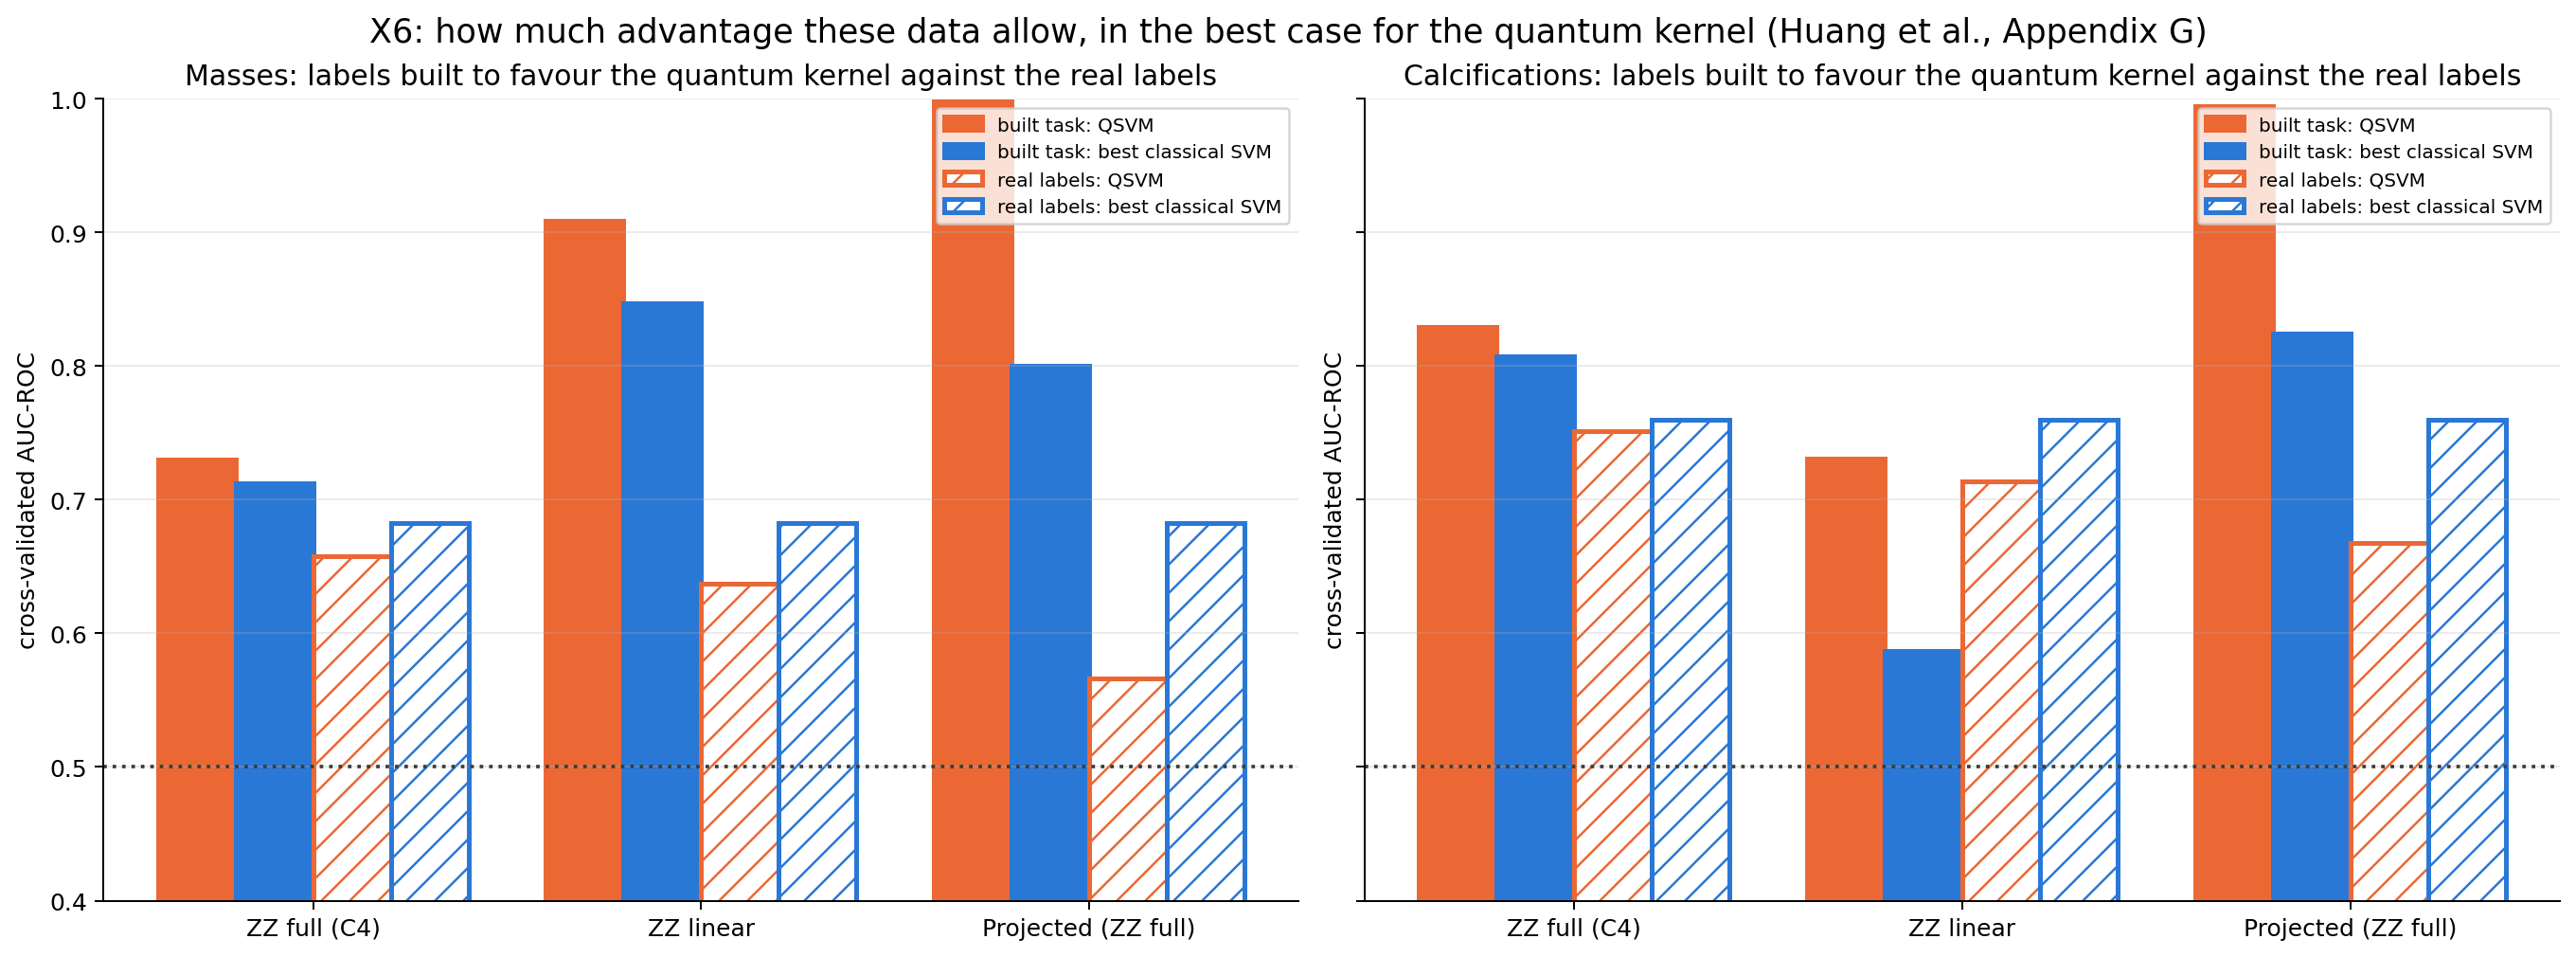
\includegraphics[width=\textwidth]{Figures/X6_built_labels.png}
\caption{Desempeño clasificatorio sobre etiquetas sintéticas diseñadas según la geometría cuántica en comparación con las etiquetas clínicas diagnósticas reales de CBIS-DDSM.}
\label{fig:x6_built_labels}
\end{figure}
